%&../../.preamble
\endofdump
\usepackage{contour}

\usetikzlibrary{external}
\tikzset{external/system call={pdflatex --shell-escape --fmt=../.preamble --halt-on-error -jobname "\image" "\endofdump\texsource"}}
\tikzexternalize[prefix=tikz/]

\title{Ripetizioni Annalisa}
\author{Marini Mattia}
\date{Ottobre 2024}

\begin{document}
\maketitle
\license{Ripetizioni Annalisa}

\tableofcontents

\newpage
\section{Conoscenze fondamentali}
\subsection{Derivate}
\renewcommand{\arraystretch}{1.4}
Qui di seguito un cheatsheet con le regole di derivazione delle funzioni fondamentali:
\begin{center}
	\begin{tabular}{l l l}
		\hline
		Nome funzione               & $ f\left(x\right) $ & $f'(x)$                     \\
		\hline
		Polinomio                   & $  x^{n} $          & $  n  x^{n-1} $             \\
		Costante                    & $  c $              & $  0 $                      \\
		Esponenziale                & $  e^{x} $          & $  e^{x} $                  \\
		Esponenziale con base $ a $ & $  a^{x} $          & $  a^{x} \ln(a) $           \\
		Logaritmo naturale          & $  \ln(x) $         & $  \frac{1}{x} $            \\
		Seno                        & $  \sin(x) $        & $  \cos(x) $                \\
		Coseno                      & $  \cos(x) $        & $  -\sin(x) $               \\
		Tangente                    & $  \tan(x) $        & $  \frac{1}{\cos^{2}(x)} $  \\
		Cotangente                  & $  \cot(x) $        & $  -\frac{1}{\sin^{2}(x)} $ \\
		\hline
	\end{tabular}
\end{center}
\renewcommand{\arraystretch}{1}
Qui di seguito un cheasheet con le regole di derivazioni per funzioni composte, prodotti e divisioni di funzioni:
\renewcommand{\arraystretch}{1.4}
\begin{center}
	\begin{tabular}{l l l}
		\hline
		Tipo operazione       & $ f\left(x\right) $    & $f '(x)$                                  \\
		\hline
		Prodotto per costante & $  cf(x) $             & $ cf'(x) $                                \\
		Prodotto fra funzioni & $  f(x)g(x) $          & $  f'(x)g(x) + f(x)g'(x) $                \\
		Quoziente             & $  \frac{f(x)}{g(x)} $ & $  \frac{f'(x)g(x) - f(x)g'(x)}{g(x)^2} $ \\
		Funzione composta     & $  f(g(x)) $           & $  f'(g(x))g'(x) $                        \\
		\hline
	\end{tabular}
\end{center}

\renewcommand{\arraystretch}{1}
\subsection{Limiti}
Per quanto riguarda i limiti è fondamentale:
\begin{itemize}
	\item Avere chiaro dal punto di vista inttuitivo il concetto di infinito, classi di infinito e di "tendere a" (avvicinarsi asintoticamente ad un valore)
	\item Sapere risolvere limiti e in particolare le forme indeterminate
\end{itemize}

\renewcommand{\arraystretch}{1.4}
\begin{center}
	\begin{tabular}{l l l}
		\hline
		Funzione             & limite                                                     & tipo F.I          \\
		\hline
		Seno                 & $ \lim_{x \to 0} \frac{\sin(x)}{x} = 1 $                   & $ [\frac{0}{0}] $ \\
		Coseno               & $ \lim_{x \to 0} \frac{1-\cos(x)}{x^2} = \frac{1}{2} $     & $ [\frac{0}{0}] $ \\
		Numero di Nepero     & $ \lim_{n \to \infty} \left(1 + \frac{1}{n}\right)^n = e $ & $ 1^{\infty } $   \\
		Esponenziale         & $ \lim_{x \to 0} \frac{e^x - 1}{x} = 1 $                   & $ [\frac{0}{0}] $ \\
		Logaritmo            & $ \lim_{x \to 0} \frac{\ln(1+x)}{x} = 1 $                  & $ [\frac{0}{0}] $ \\
		Potenza di se stessa & $ \lim_{x \to 0^+} x^x = 1 $                               & $ 0^{0} $         \\
		\hline
	\end{tabular}
\end{center}
\renewcommand{\arraystretch}{1}
NB: spesso ricondursi ad un limite notevole è più impegnativo che applicare de l'Hopital meccanicamente. L'unico caso in cui è necessario l'utilizzo di un limite notevole è quello in cui si ha $ 0^{0} $ o $ 1^{\infty } $

\subsubsection*{Cheatsheet forme indeterminate}
\vskip3mm
\begin{center}
	\begin{forest}
		for tree={draw, grow=0, align = left, child anchor=west, anchor=base
		west, tier/.pgfmath=level()}
		[Limite
		[{$ \left[\frac{0}{0}\right] $ o $ \left[\frac{\infty}{\infty }\right] $}
			[- Confronto tra classi di infinito\\
				- Raccoglimento (con polinomi)\\
				- De l'Hopital
			]
		]
		[{$ \left[0^{\infty}\right] $ o $ \left[\infty ^{0}\right]  $}
		[- {Utilizzo $ x = e^{\ln\left(x\right)} $}]
		]
		[{$ \left[1^{\infty}\right] $}
		[- Limite di Nepero\\
		- {Utilizzo $ x = e^{\ln\left(x\right)} $}
		]
		]
		[{$ \left[\infty - \infty \right] $}
			[- Razionalizzazione inversa]
		]
		]
	\end{forest}
\end{center}
\subsubsection*{Classi di infiniti}

\begin{minipage}[t]{0.48\textwidth}
	"Rapidità" con cui funzioni note tendono ad infinito (in ordine descrescente)
	\[
		\lim_{x \to \infty} f(x)
	\]
	\begin{center}
		\begin{forest}
			for tree={draw, grow = -90, edge={latex-}}
			[$ x! $ %, tikz={\node [draw, dashed, inner sep=5pt,fit to=tree, label={90:$ \lim_{x \to \infty} f(x) $}]{};}
			[$ n^{x} \rightarrow \left(n-1\right)^{x} \rightarrow e^{x} \ldots \;  3^{x} \rightarrow   2^{x} \rightarrow      $
					[$ x^{n} \rightarrow  x^{n-1} \ldots \; x^{2} \rightarrow x^{1}  $
							[{$ \sqrt{x}  \rightarrow  \sqrt[3]{x} \rightarrow  x^{\frac{1}{4}} \ldots $}
										[ {$  \log_2(x+1) \rightarrow \ln\left(x+1\right) \rightarrow  \log _3 \left(x+1\right) \ldots $}]
								]
						]
				]
			]
		\end{forest}
	\end{center}
\end{minipage}
%
\begin{minipage}[t]{0.48\textwidth}
	"Rapidità" con cui funzioni note tendono a $ 0 $ (in ordine descrescente)
	\[
		\lim_{x \to 0} f(x)
	\]
	\begin{center}
		\begin{forest}
			for tree={draw, grow = -90, edge={latex-}}
			[$ x^{n} \rightarrow  x^{n-1} \ldots \; x^{2} \rightarrow x^{1}  $
			[{$ \sqrt{x}  \rightarrow  \sqrt[3]{x} \rightarrow  x^{\frac{1}{4}} \ldots $}
						[ {$  \log_2(x) \rightarrow \ln\left(x\right) \rightarrow  \log _3 \left(x\right) \ldots $}]
				]
			]
			]
		\end{forest}
	\end{center}
\end{minipage}


\section{Punti di discontinuità}
\subsection{Discontinuità a salto finito}
Limite destro e sinistro tendono a valori finiti ma diversi tra loro:
\[
	\lim_{x \to x_0^{-}} f(x) \neq \lim_{x \to x_0^{+}} f(x) \quad \text{ esiste finito }
\]
\begin{minipage}[c]{0.48\textwidth}
	\begin{tikzpicture}
		\begin{axis}[
				xmin=-2, xmax=2,
				ymin=-4,ymax=4,
				restrict y to domain = -4:4, domain=-2:2, width=0.98\textwidth, height=0.98\textwidth, grid=major, samples=200,  ylabel=$f(x)$, xlabel=$x$]
			\addplot[black, thick, domain = -4:0] {-1};
			\addplot[black, thick, domain = 0:4] {1};
			\node [blackdot] at (0,0){};
			\node [whitedot] at (0,1){};
			\node [whitedot] at (0,-1){};
		\end{axis}
	\end{tikzpicture}
\end{minipage}
%
\begin{minipage}[c]{0.48\textwidth}
	\begin{tikzpicture}
		\begin{axis}[
				xmin=-2, xmax=2,
				ymin=-4,ymax=4,
				restrict y to domain = -4:4, domain=-2:2, width=0.98\textwidth, height=0.98\textwidth, grid=major, samples=200,  ylabel=$f(x)$, xlabel=$x$]
			\addplot[black, thick, domain = -4:0] {-1};
			\addplot[black, thick, domain = 0:4] {1};
			\node [whitedot] at (0,1){};
			\node [whitedot] at (0,-1){};
		\end{axis}
	\end{tikzpicture}
\end{minipage}
\subsection{Discontinuità di secondo tipo}
Almeno uno dei due limiti (sinistro o destro) tende a valori infiniti o non esiste:
\[
	\lim_{x \to x_0^{-}} f(x)
	\begin{cases}
		\pm \infty \\
		\not \exists
	\end{cases}
	\quad \text{ oppute } \quad
	\lim_{x \to x_0^{+}} f(x)
	\begin{cases}
		\pm \infty \\
		\not \exists
	\end{cases}
\]
\begin{minipage}[c]{0.48\textwidth}
	\[
		f\left(x \right) = \frac{x^2 + 2}{x^2 -1}
	\]

	\begin{center}
		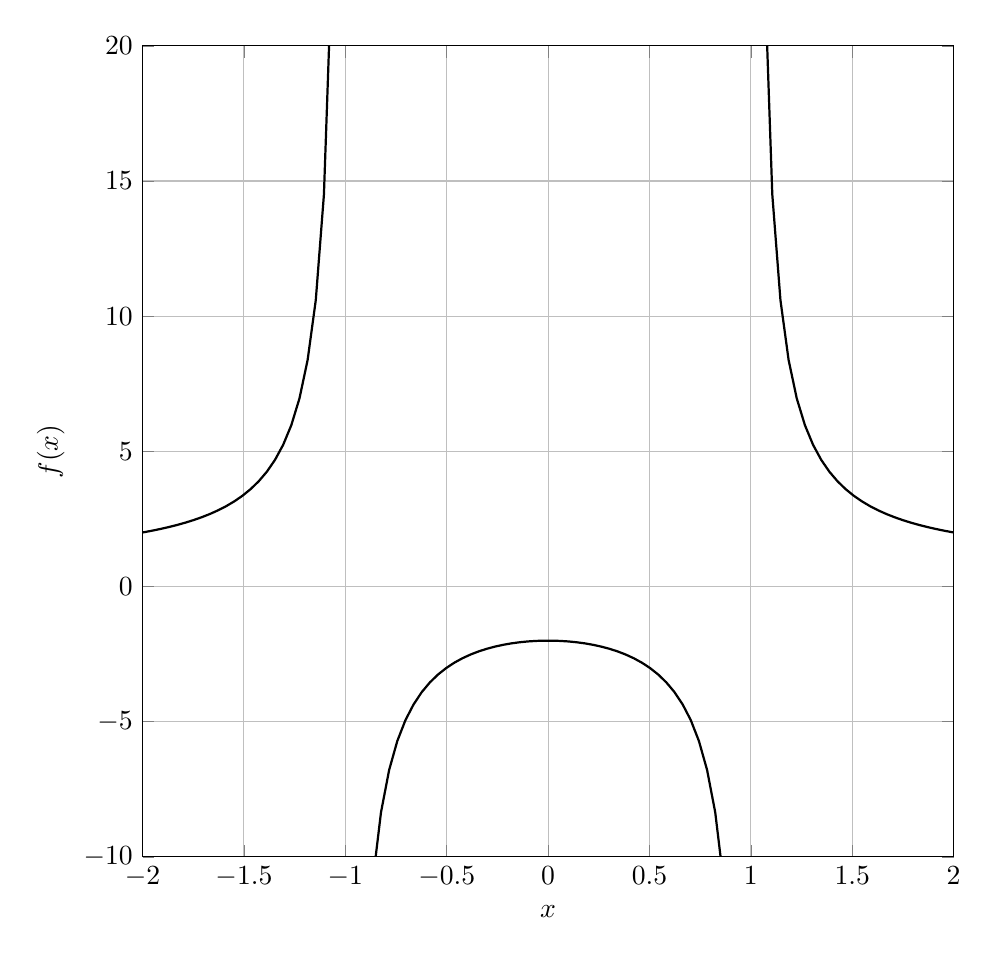
\begin{tikzpicture}
			\begin{axis}[
					xmin=-2, xmax=2,
					ymin=-10,ymax=20,
					restrict y to domain = -40:40, domain= :5, width=0.98\textwidth, height=0.98\textwidth, grid=major, samples=200,  ylabel=$f(x)$, xlabel=$x$]
				\addplot[black, thick, domain = -4:4] {(x^2+2)/(x^2-1)};
			\end{axis}
		\end{tikzpicture}
	\end{center}
\end{minipage}
%
\begin{minipage}[c]{0.48\textwidth}
	\[
		f\left(x\right)=
		\begin{cases}
			\sin \left(\frac{1}{x}\right) & x < 0   \\
			0                             & x \ge 0
		\end{cases}
	\]
	\begin{center}
		\begin{tikzpicture}
			\begin{axis}[
					xmin=-2, xmax=2,
					ymin=-2,ymax=4,
					restrict y to domain = -40:40, domain=-2:2, width=0.98\textwidth, height=0.98\textwidth, grid=major, samples=400,  ylabel=$f(x)$, xlabel=$x$]
				\addplot[black, thick, domain = -4:0] {sin(deg(1/x))};
				\addplot[black, thick, domain = 0:4] {0};
				\node [whitedot] at (0,0){};
			\end{axis}
		\end{tikzpicture}
	\end{center}
\end{minipage}

\subsection{Discontinuità eliminabile}
I limiti destro e sinitro esistono \textit{finiti} e \textit{coincidono} ma in quel punto la funzione ha vaole diverso o non è definita

\vskip3mm
\begin{minipage}[c]{0.48\textwidth}
	\[
		f\left(x \right) =
		\begin{cases}
			1 & x \neq 0 \\
			2 & x = 0
		\end{cases}
	\]

	\begin{center}
		\begin{tikzpicture}
			\begin{axis}[
					xmin=-2, xmax=2,
					ymin=0,ymax=4,
					restrict y to domain = -4:4, domain=-2:2, width=0.98\textwidth, height=0.98\textwidth, grid=major, samples=200,  ylabel=$f(x)$, xlabel=$x$]
				\addplot[black, thick, domain = -4:0] {1};
				\addplot[black, thick, domain = 0:4] {1};
				\node [blackdot] at (0,2){};
				\node [whitedot] at (0,1){};
			\end{axis}
		\end{tikzpicture}
	\end{center}
\end{minipage}
%
\begin{minipage}[c]{0.48\textwidth}
	\[
		f\left(x\right)=
		\frac{\sin\left(x\right)}{x}
	\]
	\begin{center}
		\begin{tikzpicture}
			\begin{axis}[
					xmin=-10, xmax=10,
					ymin=-2,ymax=2,
					restrict y to domain = -40:40, domain=-10:10, width=0.98\textwidth, height=0.98\textwidth, grid=major, samples=400,  ylabel=$f(x)$, xlabel=$x$]
				\addplot[black, thick] {sin(deg(x))/x};
				\node [whitedot] at (0,1){};
			\end{axis}
		\end{tikzpicture}
	\end{center}
\end{minipage}

La discontinuità è detta eliminabile in quanto è possibile rendere la funzione continua modificando solamente il punto in cui questa presenta la discontinuità stessa, facendolo coincidere con il limite destro e sinistro

\section{Punti di non derivabilità}
\subsection{Punto angoloso}
Il limite destro e sinistro della derivata prima sono valori finiti ma non coincidono
\vskip3mm
\begin{minipage}[t]{0.48\textwidth}
	\[
		f\left(x\right) = \left|x\right|
	\]
	\begin{center}
		\begin{tikzpicture}
			\begin{axis}[
					xmin=-2, xmax=2,
					ymin=-1,ymax=3,
					restrict y to domain = -4:4, domain=-2:2, width=0.98\textwidth, height=0.98\textwidth, grid=major, samples=200,  ylabel=$f(x)$, xlabel=$x$]
				\addplot[black, thick] {abs(x)};
				\node [blackdot] at (0,0){};
			\end{axis}
		\end{tikzpicture}
	\end{center}
\end{minipage}
%
\begin{minipage}[t]{0.48\textwidth}
	\[
		f\left(x\right)= \left|\ln\left(x\right)\right|
	\]
	\begin{center}
		\begin{tikzpicture}
			\begin{axis}[
					xmin=-2, xmax=6,
					ymin=-1,ymax=3,
					restrict y to domain = -40:40, domain=-10:10, width=0.98\textwidth, height=0.98\textwidth, grid=major, samples=400,  ylabel=$f(x)$, xlabel=$x$]
				\addplot[black, thick] {abs(ln(x))};
				\node [blackdot] at (1,0){};
			\end{axis}
		\end{tikzpicture}
	\end{center}
\end{minipage}
\subsection{Cuspide}
Il limite destro e sinistro della derivata prima sono \textit{infiniti di segno opposto}
\vskip3mm
\begin{minipage}[t]{0.48\textwidth}
	\[
		f\left(x\right) = \left|x\right|
	\]
	\begin{center}
		\begin{tikzpicture}
			\begin{axis}[
					xmin=-2, xmax=2,
					ymin=-1,ymax=3,
					restrict y to domain = -4:4, domain=-2:2, width=0.98\textwidth, height=0.98\textwidth, grid=major, samples=200,  ylabel=$f(x)$, xlabel=$x$]
				\addplot[black, thick] {sqrt(abs(x))};
				\node [blackdot] at (0,0){};
			\end{axis}
		\end{tikzpicture}
	\end{center}
\end{minipage}
%
\begin{minipage}[t]{0.48\textwidth}
	\[
		f\left(x\right) = \sqrt[3]{\left(x-1\right)^2 }
	\]
	\begin{center}
		\begin{tikzpicture}
			\begin{axis}[
					xmin=-2, xmax=6,
					ymin=-1,ymax=3,
					restrict y to domain = -40:40, domain=-10:10, width=0.98\textwidth, height=0.98\textwidth, grid=major, samples=400,  ylabel=$f(x)$, xlabel=$x$]
				\addplot[black, thick] {((x-1)^2)^(1/3)};
				\node [blackdot] at (1,0){};
			\end{axis}
		\end{tikzpicture}
	\end{center}
\end{minipage}
\subsection{Flesso a tangenza verticale}

\vskip3mm
\begin{minipage}[t]{0.48\textwidth}
	\[
		f\left(x\right) = \sqrt[3]{x}
	\]
	\begin{center}
		\begin{tikzpicture}
			\begin{axis}[
					xmin=-2, xmax=2,
					ymin=-2,ymax=2,
					restrict y to domain = -4:4, domain=-2:2, width=0.98\textwidth, height=0.98\textwidth, grid=major, samples=200,  ylabel=$f(x)$, xlabel=$x$]
				\addplot[black, thick] {sign(x)*(abs(x))^(1/3)};
				\node [blackdot] at (0,0){};
			\end{axis}
		\end{tikzpicture}
	\end{center}
\end{minipage}
%
\begin{minipage}[t]{0.48\textwidth}
	\[
		f\left(x\right) = \sqrt[3]{\frac{\left(x-1\right)}{2} }
	\]
	\begin{center}
		\begin{tikzpicture}
			\begin{axis}[
					xmin=-2, xmax=6,
					ymin=-1,ymax=3,
					restrict y to domain = -40:40, domain=-10:10, width=0.98\textwidth, height=0.98\textwidth, grid=major, samples=400,  ylabel=$f(x)$, xlabel=$x$]
				\addplot[black, thick] {sign(0.5*(x-1))*(abs(0.5*(x-1)))^(1/3)};
				\node [blackdot] at (1,0){};
			\end{axis}
		\end{tikzpicture}
	\end{center}
\end{minipage}
\subsection{Casi particolari}
Oltre ai casi sopra citati, vi sono casi particolari in cui non è possibile parlare di derivata di una funzione. Il seguente è quello più comune:
\[
	f\left(x\right) = \sin \left(\frac{1}{x}\right)
\]

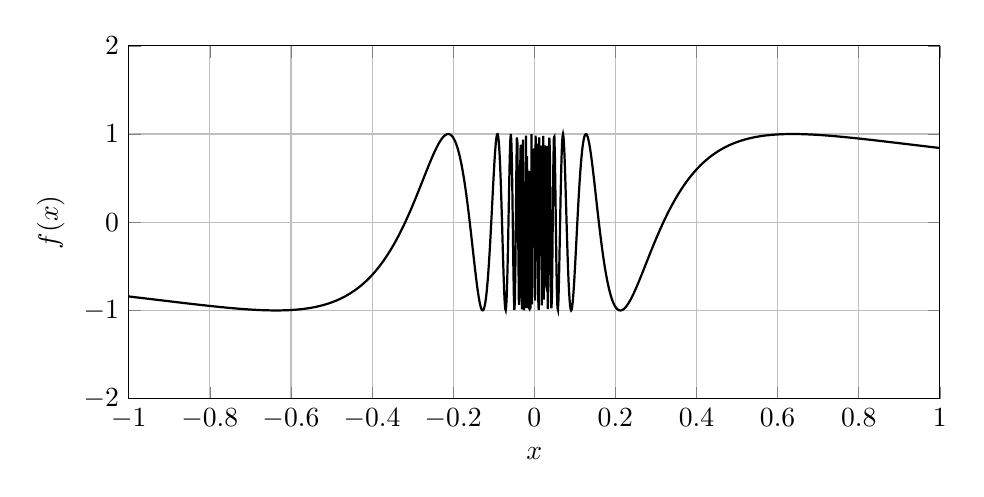
\begin{tikzpicture}
	\begin{axis}[
			xmin=-1, xmax=1,
			ymin=-2,ymax=2,
			restrict y to domain = -2:2, domain=-5:5, width=0.98\textwidth, height=0.5\textwidth, grid=major, samples=8000,  ylabel=$f(x)$, xlabel=$x$]
		\addplot[black, thick] {sin(deg(1/x))};
	\end{axis}
\end{tikzpicture}
Avvicinandosi all'origine, la funzione oscilla sempre più rapidamente, dunque la sua derivata non tende a nessun valore, ma oscillerà sempre più velocemente anch'essa
\section{Esercizi preliminari studio di funzione}
\begin{esercizio}{Classicifa punti discontinuità (p. 1560 n. 853)}
	Data la funzione
	\[
		f\left(x\right) =
		\begin{cases}
			2x                 & \text{ se } x \le 1 \\
			ln\left(x-1\right) & \text{ se } x > 1
		\end{cases}
	\]
	calcolane i punti di discontinuità e nel casi siano di prima specie, calcolane il salto
\end{esercizio}

\subsubsection*{Soluzione}
Il dominio di $ 2x $ è $ \R  $, mentre il dominio di $ \ln\left(x-1\right) $ è $ {x \in \R \text{ t.c. } x > 1} $. Il dominio di $ f\left(x\right) $ è dunque:
\[
	\R - \left\{1\right\}
\]
\vskip3mm
I limiti destro e sinistro valgono:
\begin{align*}
	\lim_{x \to 1^{+}} f(x) & = \lim_{x \to 1^{+}} ln\left(x-1\right) = -\infty \\
	\lim_{x \to 1^{-}} f(x) & = \lim_{x \to 1^{-}} 2x = 2
\end{align*}
rientriamo dunque nel caso della \textit{discontinuità di secondo tipo}

\begin{tikzpicture}
	\begin{axis}[
			xmin=-5, xmax=5,
			ymin=-5,ymax=5,
			restrict y to domain = -50:50, domain=-5:5, width=0.98\textwidth, height=0.48\textwidth, grid=major, samples=200,  ylabel=$f(x)$, xlabel=$x$, legend entries={$f\left(x\right)$}]
		\addplot[black, thick, domain=-5:1] {2*x};
		\addplot[black, thick, domain=1:5] {ln(x-1)};
		\node [blackdot] at (1,2,){};
	\end{axis}
\end{tikzpicture}


\begin{esercizio}{Classicifa punti discontinuità (p. 1561 n. 856)}
	Data la funzione
	\[
		f\left(x\right) = \frac{2 \left|x\right|}{x} -3
	\]
	calcolane i punti di discontinuità e nel casi siano di prima specie, calcolane il salto
\end{esercizio}
\begin{tikzpicture}
	\begin{axis}[
			xmin=-5, xmax=5,
			ymin=-6,ymax=2,
			restrict y to domain = -10:10, domain=-5:5, width=0.98\textwidth, height=0.5\textwidth, grid=major, samples=200,  ylabel=$f(x)$, xlabel=$x$, legend entries={$ $}]
		\addplot[black, thick, domain=-5:0] {(2*sign(x)-3};
		\addplot[black, thick, domain=0:5] {(1-3};
		\node [whitedot] at (0,-2){};
		\node [whitedot] at (0,-5){};
	\end{axis}
\end{tikzpicture}


\begin{esercizio}{Classicifa punti discontinuità (p. 1561 n. 871)}
	Data la funzione
	\[
		f\left(x\right) = \frac{\sin \left(x\right)}{\sin \left(2x\right)}
	\]
	calcolane i punti di discontinuità e nel casi siano di prima specie, calcolane il salto
\end{esercizio}
Qui la situazione è un po' più complicata in quanto dal dominio vanno esclusi tutti e soli i valori che annullano il denominatore. Essendo quest'ultimo una funzione trigonometrica, avremo infiniti valori per i quali questo sarà nullo. Partiamo imponento il denominatore $ = 0 $:
\[
	\sin \left(2x\right) = 0 \rightarrow 2x = k \pi \rightarrow x = \frac{k \pi }{2} \quad \text{ dove }  k  \in \N
\]
Prendiamo ora due punti $ x_1 $ e $ x_2 $ esclusi dal dominio e studiamo il comportamento della funzione nel loro intorno:
\[
	x_1 = \frac{1 \cdot  \pi }{2} = \frac{\pi}{2} \quad \quad x_2 = \frac{2 \pi }{2} = \pi
\]
calcoliamo limite destro e sinistro:
\[
	\lim_{x \to x_1^{-}} f(x) = \lim_{x \to x_1^{-}} \frac{\sin \left(x\right)}{\sin \left(2x\right)} = \left[ \frac{\sin \left( \frac{\pi }{2}\right)}{ \sin \left(\pi \right)} \right] = \left[\frac{1}{0^{+}}\right] = +\infty
\]

\[
	\lim_{x \to x_1^{+}} f(x) = \lim_{x \to x_1^{-}} \frac{\sin \left(x\right)}{\sin \left(2x\right)} = \left[ \frac{\sin \left( \frac{\pi }{2}\right)}{ \sin \left(\pi \right)} \right] = \left[\frac{1}{0^{-}}\right] = -\infty
\]
facendo la stessa cosa con $ x_2 $ ottengo una forma indeterminata che posso risolvere riscrivendo l'espressione così:
\[
	\frac{\sin \left(x\right)}{\sin \left(2x\right)}  = \frac{\sin \left(x\right)}{2 \sin \left(x\right) \cos \left(x\right)} = \frac{1}{2 \cos\left(x\right)}
\]
dunque facendo il limite
\[
	\lim_{x \to x_2}  \frac{1}{2 \cos }  = \left[ \frac{1}{2 \cos \left(\pi \right)}\right] = \frac{1}{2}
\]
\vskip3mm
Il risultato è dunque interessante: ottengo un punto di discontinuità di secondo tipo per ogni $ k $ \textit{dispari}, mentre un punto di discontinuità eliminabile per ogni $ k $ \textit{pari}

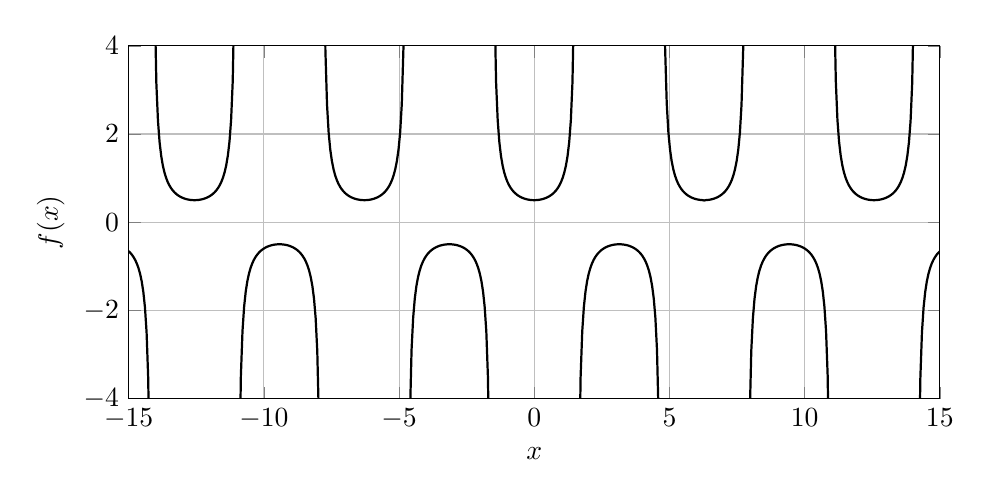
\begin{tikzpicture}
	\begin{axis}[
			xmin=-15, xmax=15,
			ymin=-4,ymax=4,
			restrict y to domain = -20:20, domain=-15:15, width=0.98\textwidth, height=0.5\textwidth, grid=major, samples=500,  ylabel=$f(x)$, xlabel=$x$]
		\addplot[black, thick] {sin(deg(x))/sin(deg(2*x))};
	\end{axis}
\end{tikzpicture}

\begin{esercizio}{Individua gli asintoti (p. 1565 n.939)}
	Individua asintoti orizzontali e verticali della seguente funzione
	\[
		f\left(x\right) = \ln\left(\frac{x+1}{x + 3}\right)
	\]
\end{esercizio}
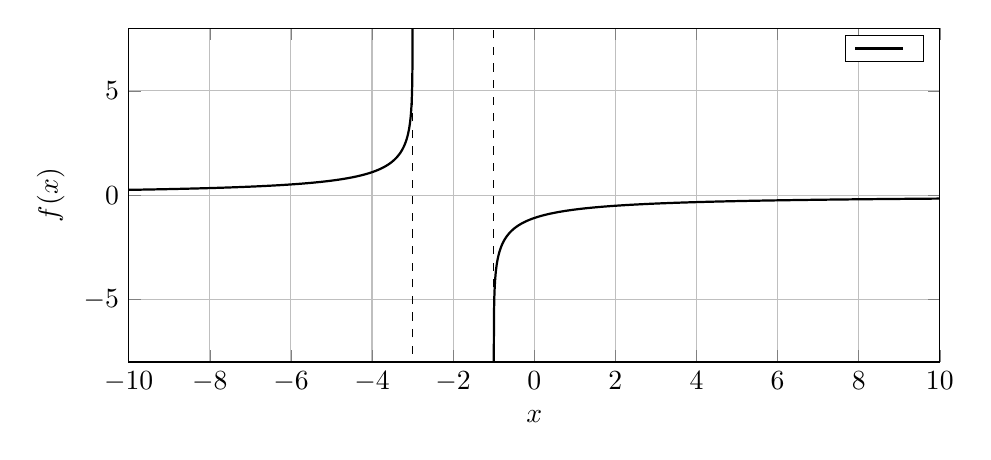
\begin{tikzpicture}
	\begin{axis}[
			xmin=-10, xmax=10,
			ymin=-8,ymax=8,
			restrict y to domain = -8000:8000, domain=-10:10, width=0.98\textwidth, height=0.48\textwidth, grid=major, samples=1800,  ylabel=$f(x)$, xlabel=$x$, legend entries={$ $}]
		\addplot[black, thick, domain=-10:-3] {ln((x+1)/(x+3))};
		\addplot[black, thick, domain=-2:10] {ln((x+1)/(x+3))};
		\draw [dashed] (-3,-10)--(-3,10);
		\draw [dashed] (-1,-10)--(-1,10);
	\end{axis}
\end{tikzpicture}

\begin{esercizio}{Individua gli asintoti (p. 1567 n.964)}
	Individua asintoti obliqui della seguente funzione
	\[
		f\left(x\right) = x + e^{-x} +1
	\]
\end{esercizio}
Si tratta di risolvere due limiti. Trovo $ m $
\[
	\lim_{x \to \infty} \frac{f(x)}{x} = \lim_{x \to \infty} \frac{x + e^{-x} + 1}{x} = 1
\]
trovo $ c $:
\[
	\lim_{x \to \infty} f(x) - mx = \lim_{x \to \infty} x + e^{-x} + 1 - x = 1
\]
quindi $ m = 1 $ e $ c = 1 $. L'equazione dell'asintoto obliquo è $ y = x + 1 $

\section{Studio di funzione}
\subsection{Teoria}
In ogni studio di funzione è opportuno affrontare i seguenti passaggi nell'ordine indicato, ottenendo passo per passo un grafico approssimato
\begin{enumerate}
	\item \textit{Dominio}
	      \begin{itemize}
		      \item Trovo valori per i quali la funzione non ha senso
	      \end{itemize}
	\item \textit{Segno}
	      \begin{itemize}
		      \item Risolvo equazione associata
		      \item Trovo zeri e intervalli in cui la funzione è positiva o negativa
	      \end{itemize}
	\item \textit{Limiti}
	      \begin{itemize}
		      \item Vedo come funzione si comporta a $ \pm \infty $ $ \rightarrow \lim_{x \to \pm \infty} f(x) $:
		      \item Vedo come funzione si comporta ad estremi del dominio e in punti esculsi dal dominio
		      \item Trovo asintoti orizzontali, verticali ed obliqui
		            \begin{itemize}
			            \item Verticali: se $ \lim_{x \to x_0} f(x) = \pm \infty  $ dove $ x_0 $ è un punto escluso dal dominio
			            \item Orizzontali: se $ \lim_{x \to \pm\infty} f(x) = k $, dove $ k $ è numero finito
			            \item Obliqui: se $ \lim_{x \to \pm\infty} \frac{f(x)}{x} = m $ dove $ m $ è finino ed è il coefficiente angolare della retta asintoto. Il quozioente di tale retta è : $ \lim_{x \to \pm \infty} \left[f(x) - mx\right] $
		            \end{itemize}
	      \end{itemize}
	\item \textit{Derivata prima}
	      \begin{itemize}
		      \item se $ f'\left(x\right) > 0 $ allora $ f $ cresce
		      \item se $ f'\left(x\right) < 0 $ allora $ f $ decresce
		      \item se $ f'\left(x\right) = 0 $ allora ho 3 opzioni:
		            \begin{itemize}
			            \item Punto di minimo locale/assoluto
			            \item Punto di massimo locale/assoluto
			            \item Flesso a tangenza orizzontale
		            \end{itemize}
	      \end{itemize}
	\item \textit{Derivata seconda}
	      \begin{itemize}
		      \item se $ f''\left(x\right) > 0 $ allora $ f $ ha concavità verso l'alto
		      \item se $ f''\left(x\right) < $ allora $ f $ ha concavità verso il basso
		      \item se $ f''\left(x\right) = 0 $ allora non si può dire nulla
	      \end{itemize}
\end{enumerate}
\subsection{Esercizi}
\begin{esercizio}{Studio di funzione}
	Studia la seguente funzione:
	\[
		x ln\left(x^2 \right)
	\]
\end{esercizio}
\begin{tikzpicture}
	\begin{axis}[
			xmin=-4, xmax=4,
			ymin=-2,ymax=2,
			restrict y to domain = -4:4, domain=-4:4, width=0.9\textwidth, height=0.9\textwidth, grid=major, samples=200,  ylabel=$f(x)$, xlabel=$x$, legend entries={$ $}]
		\addplot[black, thick] {x * ln(x^2)};
		\node (m1)[blackdot, label={90:$ m_1 $}] at (-0.38, {(-0.38) * ln((-0.38)^2)}) {};
		\node (m2)[blackdot, label={90:$ m_2 $}] at (0.38, {0.38 * ln(0.38^2)}) {};
		%
		\node [whitedot] at (0, {0 * ln(0^2)}) {};
		%
		\node [blackdot, label={110:$ x_0 $}] at (-1, {(-1) * ln((-1)^2)}) {};
		\node [blackdot, label={110:$ x_1 $}] at (1, {1 * ln(1^2)}) {};
	\end{axis}
\end{tikzpicture}
\vskip3mm
\begin{itemize}
	\item $ f'\left(x\right) = ln\left(x^2 \right) + 2 $
	\item $ f''\left(x\right) = \frac{2}{x} $
	\item No asintoti
\end{itemize}


\begin{esercizio}{Studio di funzione}
	Studia la seguente funzione:
	\[
		\frac{x^2  + 1}{x}
	\]
\end{esercizio}

\begin{tikzpicture}
	\begin{axis}[
			xmin=-10, xmax=10,
			ymin=-8,ymax=8,
			restrict y to domain = -40:40, domain=-10:10, width=0.9\textwidth, height=0.9\textwidth, grid=major, samples=201,  ylabel=$f(x)$, xlabel=$x$, legend entries={$ $}, unbounded coords=jump]
		\addplot[black, thick] {(x^2 + 1)/x};
		\addplot[dashed] {x};
		\node [blackdot, label={90:$ M $}] at (-1, {((-1)^2 + 1)/(-1)}) {};
		\node [blackdot, label={-90:$ m $}] at (1, {(1^2 + 1)/1}) {};
		\draw [dashed](0,-8)--(0,8);
	\end{axis}
\end{tikzpicture}
\begin{itemize}
	\item $ f'\left(x\right) = \frac{x^2 -1}{x^2 } $
	\item $ f''\left(x\right) = \frac{2}{x^3} $
	\item Asintoto verticale $ x=0 $ e obliquo $ y = x $
\end{itemize}
\vskip3mm

\end{document}

